\documentclass{article}
\usepackage[utf8]{inputenc}
\usepackage{graphicx}
\usepackage{enumerate}
\usepackage{amsmath}

\graphicspath{ {../figs/} }

\setlength{\parindent}{4em}
\setlength{\parskip}{1em}
\renewcommand{\baselinestretch}{1.3}

\makeatletter
% we use \prefix@<level> only if it is defined
\renewcommand{\@seccntformat}[1]{%
  \ifcsname prefix@#1\endcsname
    \csname prefix@#1\endcsname
  \else
    \csname the#1\endcsname\quad
  \fi}
% define \prefix@section
\newcommand\prefix@section{Part \thesection: }
\makeatother

\title{Lab04: Finite Differences for ODE}
\author{Prithvi Thakur}
\date{Oct 30, 2018}

\begin{document}

\maketitle

% Problem 1
\section{Computing finite difference second derivatives}
We compute the second derivative of $u(x) = 1 - x^2$ using finite differences. Since we know the value of $u$ is $0$ at the boundaries $x = \pm 1$, we can substitute these values to the first and last equation and get rid of those equations. We only compute the finite difference matrix at the inner points to obtain the solution.

\renewcommand{\theenumi}{\alph{enumi}}
\begin{enumerate}

    \item Discretize the domain into $N$ evenly spaced points between $-1\le x\le 1$.

    \item Construct a second difference operator K.
        \begin{verbatim}
            K = (-2*np.eye(N) + 
                np.diag(np.ones(N-1),k=1) + 
                np.diag(np.ones(N-1),k=-1))/dx**2
        \end{verbatim}

    \item If we evaluate the matrix product $K*u$, we see that it works at all the points except the first and the last element. This is because we do not have an expression for the second derivative of the function inside the domain at the boundaries.

    \item In this problem, we know the values of $u$ at the domain boundaries $x = \pm 1$. Therefore, we can substitute the values at these boundaries in the finite difference equations to eliminate the first and the last rows of the matrix. Therefore, we have a matrix of size $(N-2)\times(N-2)$ and we can compute the inverse to obtain the second derivative. 

    The centered finite difference stencil for the double derivative is:
    $$
    \frac{u_{i-\Delta x} - 2u_i + u_{i+\Delta x}}{\Delta x^2} = \frac{d^2u}{dx^2}
    $$
    
    In the matrix form, after removing the boundary rows and columns, we can write it as:
    
    \begin{bmatrix}
        -2 & 1 & 0 & \dots & 0 \\
        1 & -2 & 1 & \dots & 0 \\
        0 & 1 & -2 & 1 & \dots \\
        \vdots & \vdots & \vdots & \vdots & \ddots \\
        0 & 0 &\dots & 1 & -2
    \end{bmatrix}
    \begin{bmatrix}
        u_1 \\
        u_2 \\
        \vdots \\
        u_{N-3} \\
        u_{N-2}
    \end{bmatrix} 
    =
    \begin{bmatrix}
        -2 \\
        -2 \\
        -2 \\
        -2 \\
        -2 \\
    \end{bmatrix}


    \item The finite difference approximation is pretty straight forward for the above equation $u(x) = 1 - x^2$, and the double derivative is exactly equal to $-2$.

    \item For the equation $(1 - x^2)^2$, the analytical solution is $12x^2 - 4$. The numerical solution computed over 100 points is shown below.  
        
        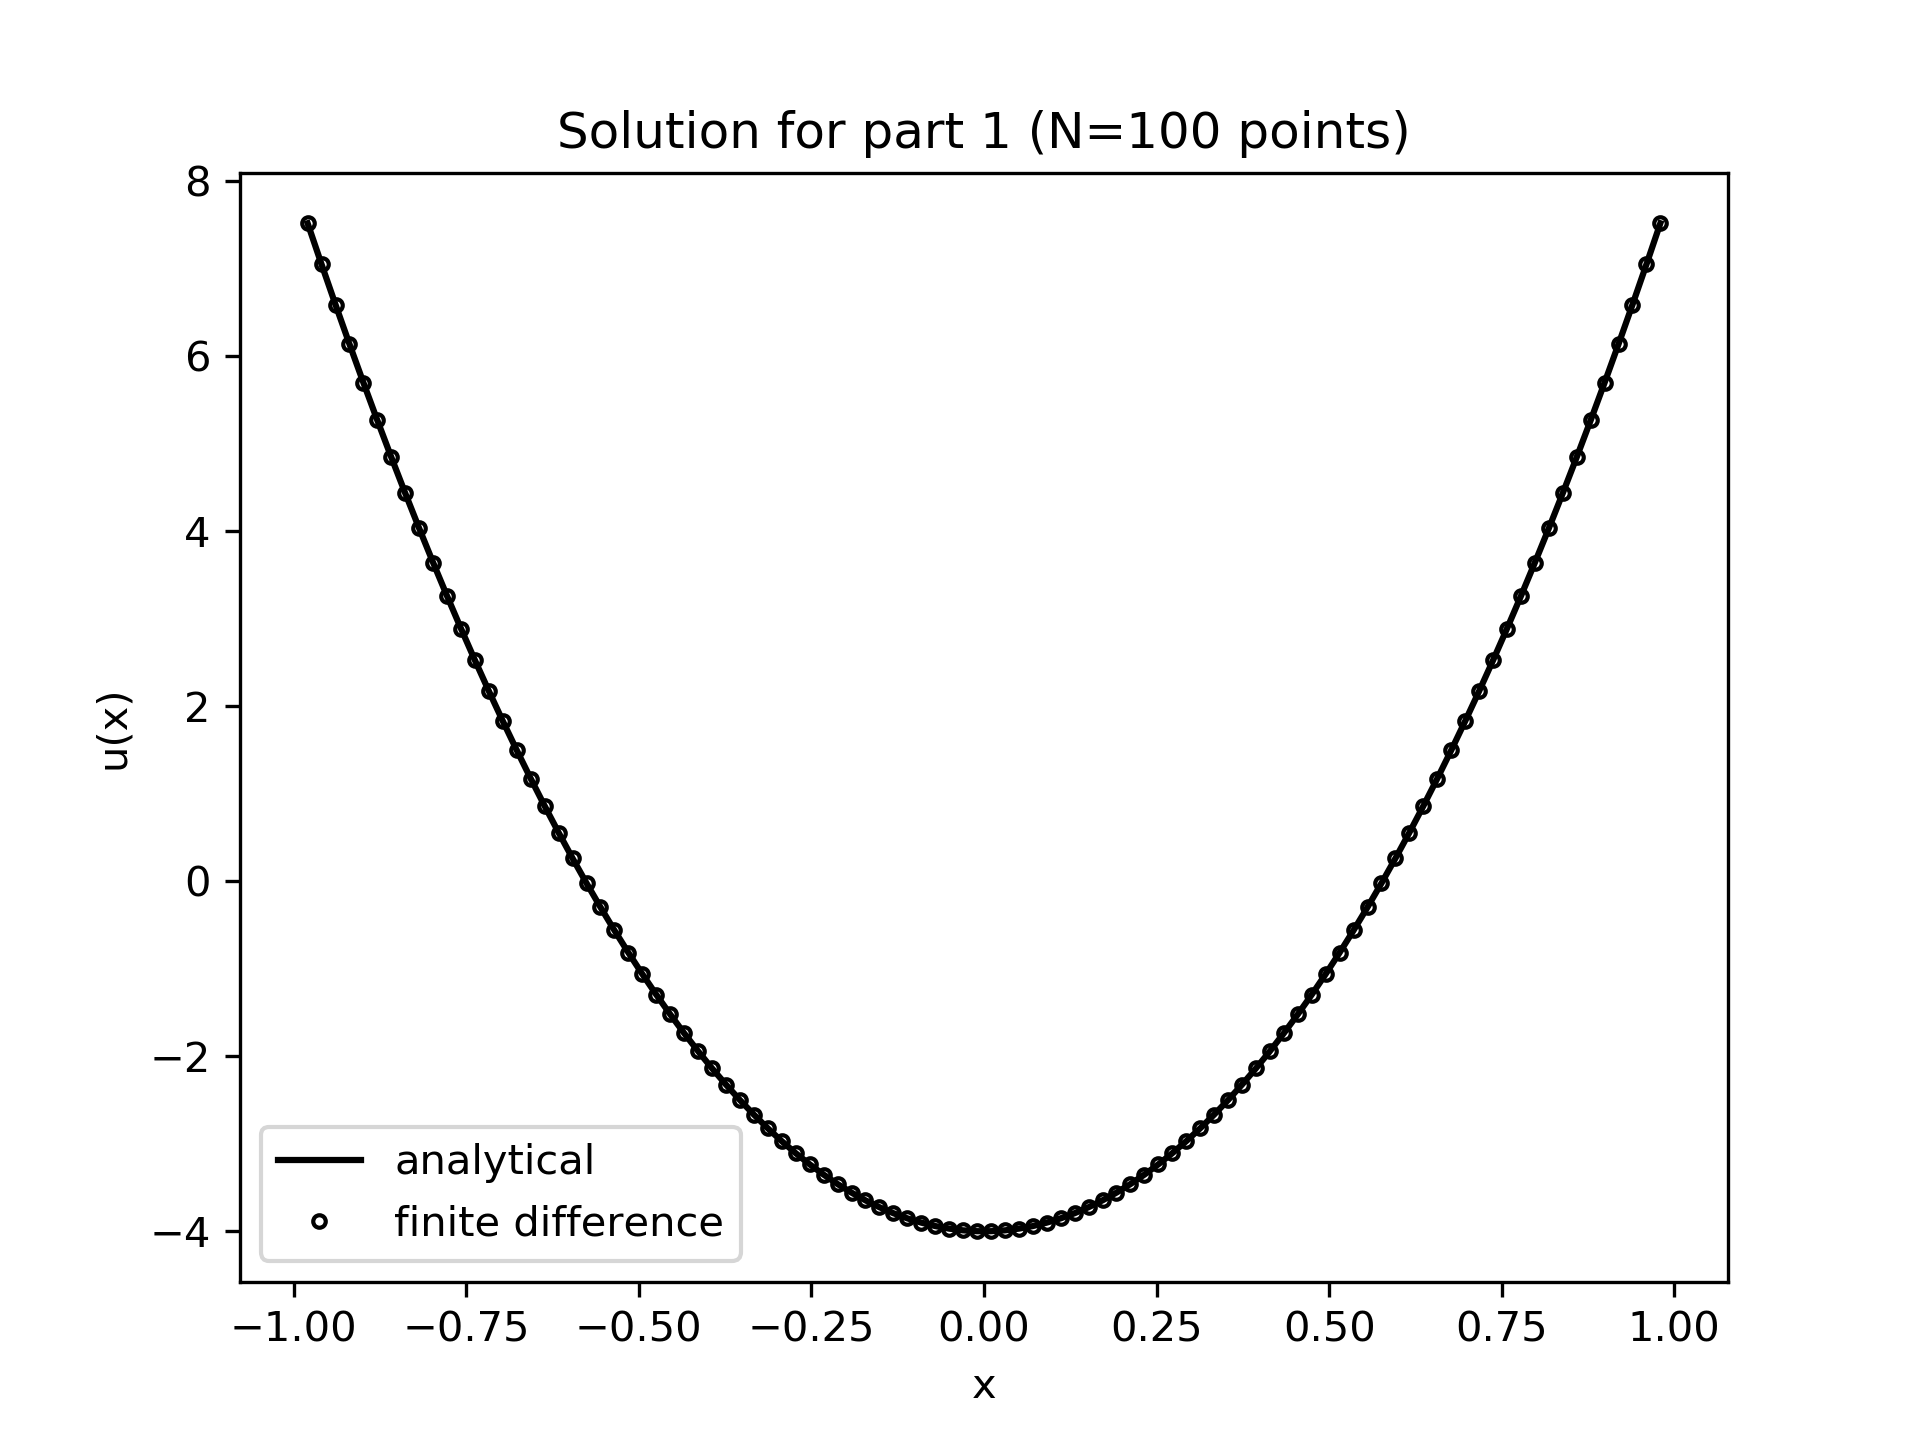
\includegraphics[scale=0.8]{part1.png}


\end{enumerate}

% Problem 2
\section{Solving Differential equations}
For the given equation and boudary conditions,

\[ -\frac{d^2u(x)}{dx^2} = 2;\  u(\pm 1) = 0 \]

The analytical solution is $u(x) = 1 - x^2$. To compute the numerical finite difference solution, we assemble a similar matrix as above with appropriate boundary conditions (which would vanish in this case since it is implicitly fulfiled), and solve for the unknown $u$ by inverting the matrix.
        
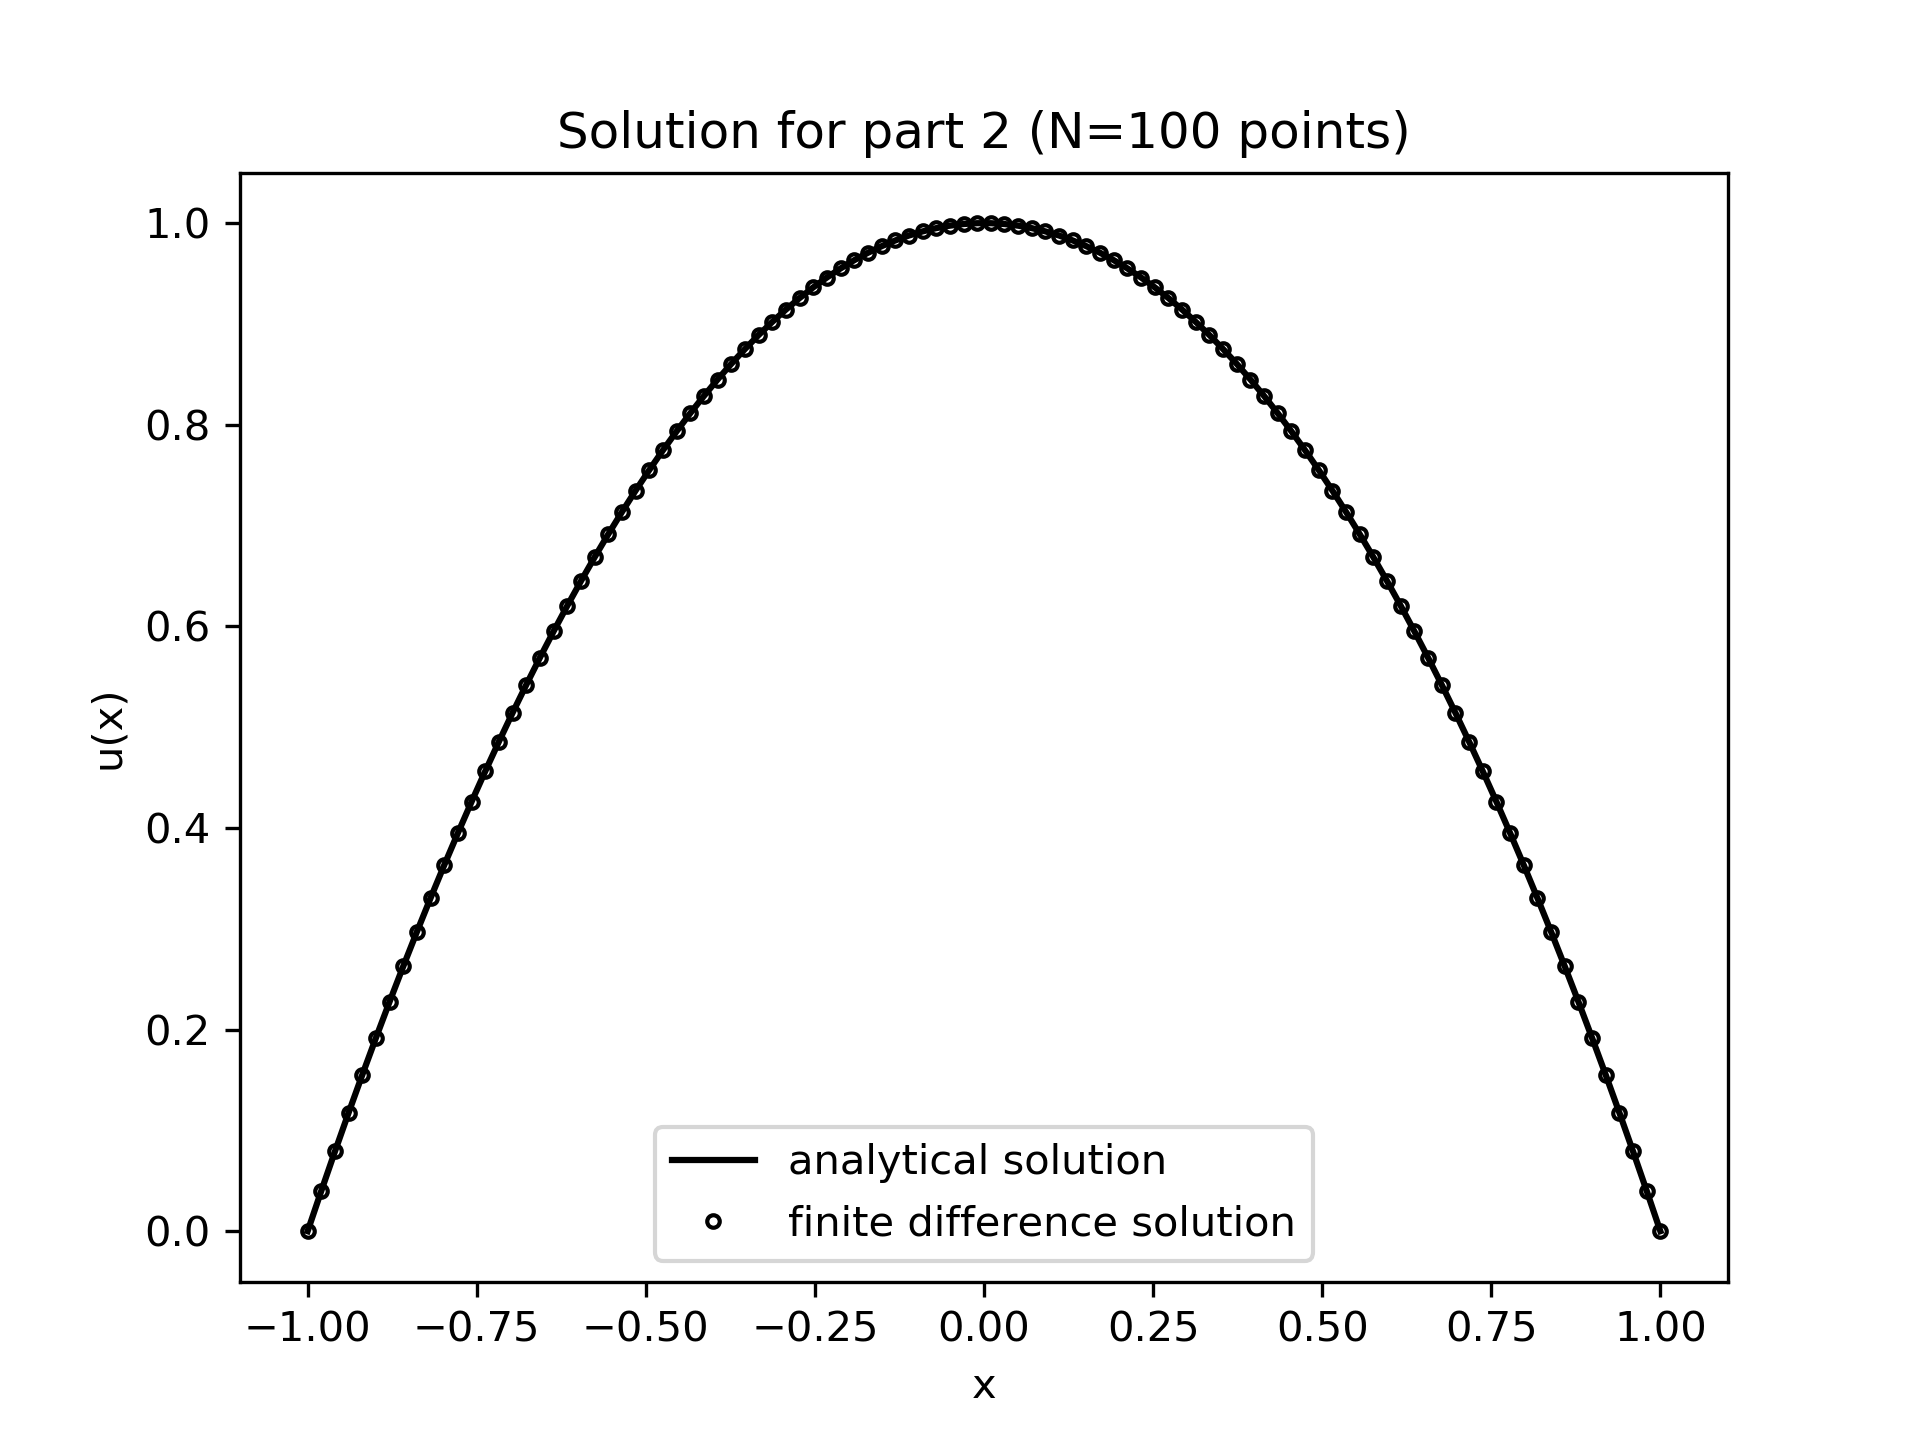
\includegraphics[scale=0.8]{part2.png}

\section{Zero slope boundary conditions}

For the same set of equations but with zero slope initial boundary condition, we will not strip the boundary rows and columns of the matrix. Since one of the boundary conditions at $x = 1$ is the same as above, we can strip off the last column and bottom row of our finite difference matrix. For the first row of our finite difference matrix, we replace the equation with the appropriate boundary condition: $\frac{du}{dx} = 0$ at $x = -1$. The finite difference discretized equation would be $\frac{u_1 - u_0}{\Delta x} = 0$. Thus our right hand side of the matrix would be zero, while the left hand coefficient would just be $1, -1$ for the first row.
    
    \begin{bmatrix}
        -1 & 1 & 0 & \dots & 0 \\
        1 & -2 & 1 & \dots & 0 \\
        0 & 1 & -2 & 1 & \dots \\
        \vdots & \vdots & \vdots & \vdots & \ddots \\
        0 & 0 &\dots & 1 & -2
    \end{bmatrix}
    \begin{bmatrix}
        u_0 \\
        u_1 \\
        \vdots \\
        u_{N-2} \\
        u_{N-1}
    \end{bmatrix} 
    =
    \begin{bmatrix}
        0 \\
        -2 \\
        -2 \\
        -2 \\
        -2 \\
    \end{bmatrix}

    The analytical vs numerical solution is shown below. The left hand side of the curve is less accurate because we use one sided finite difference for the boundary.

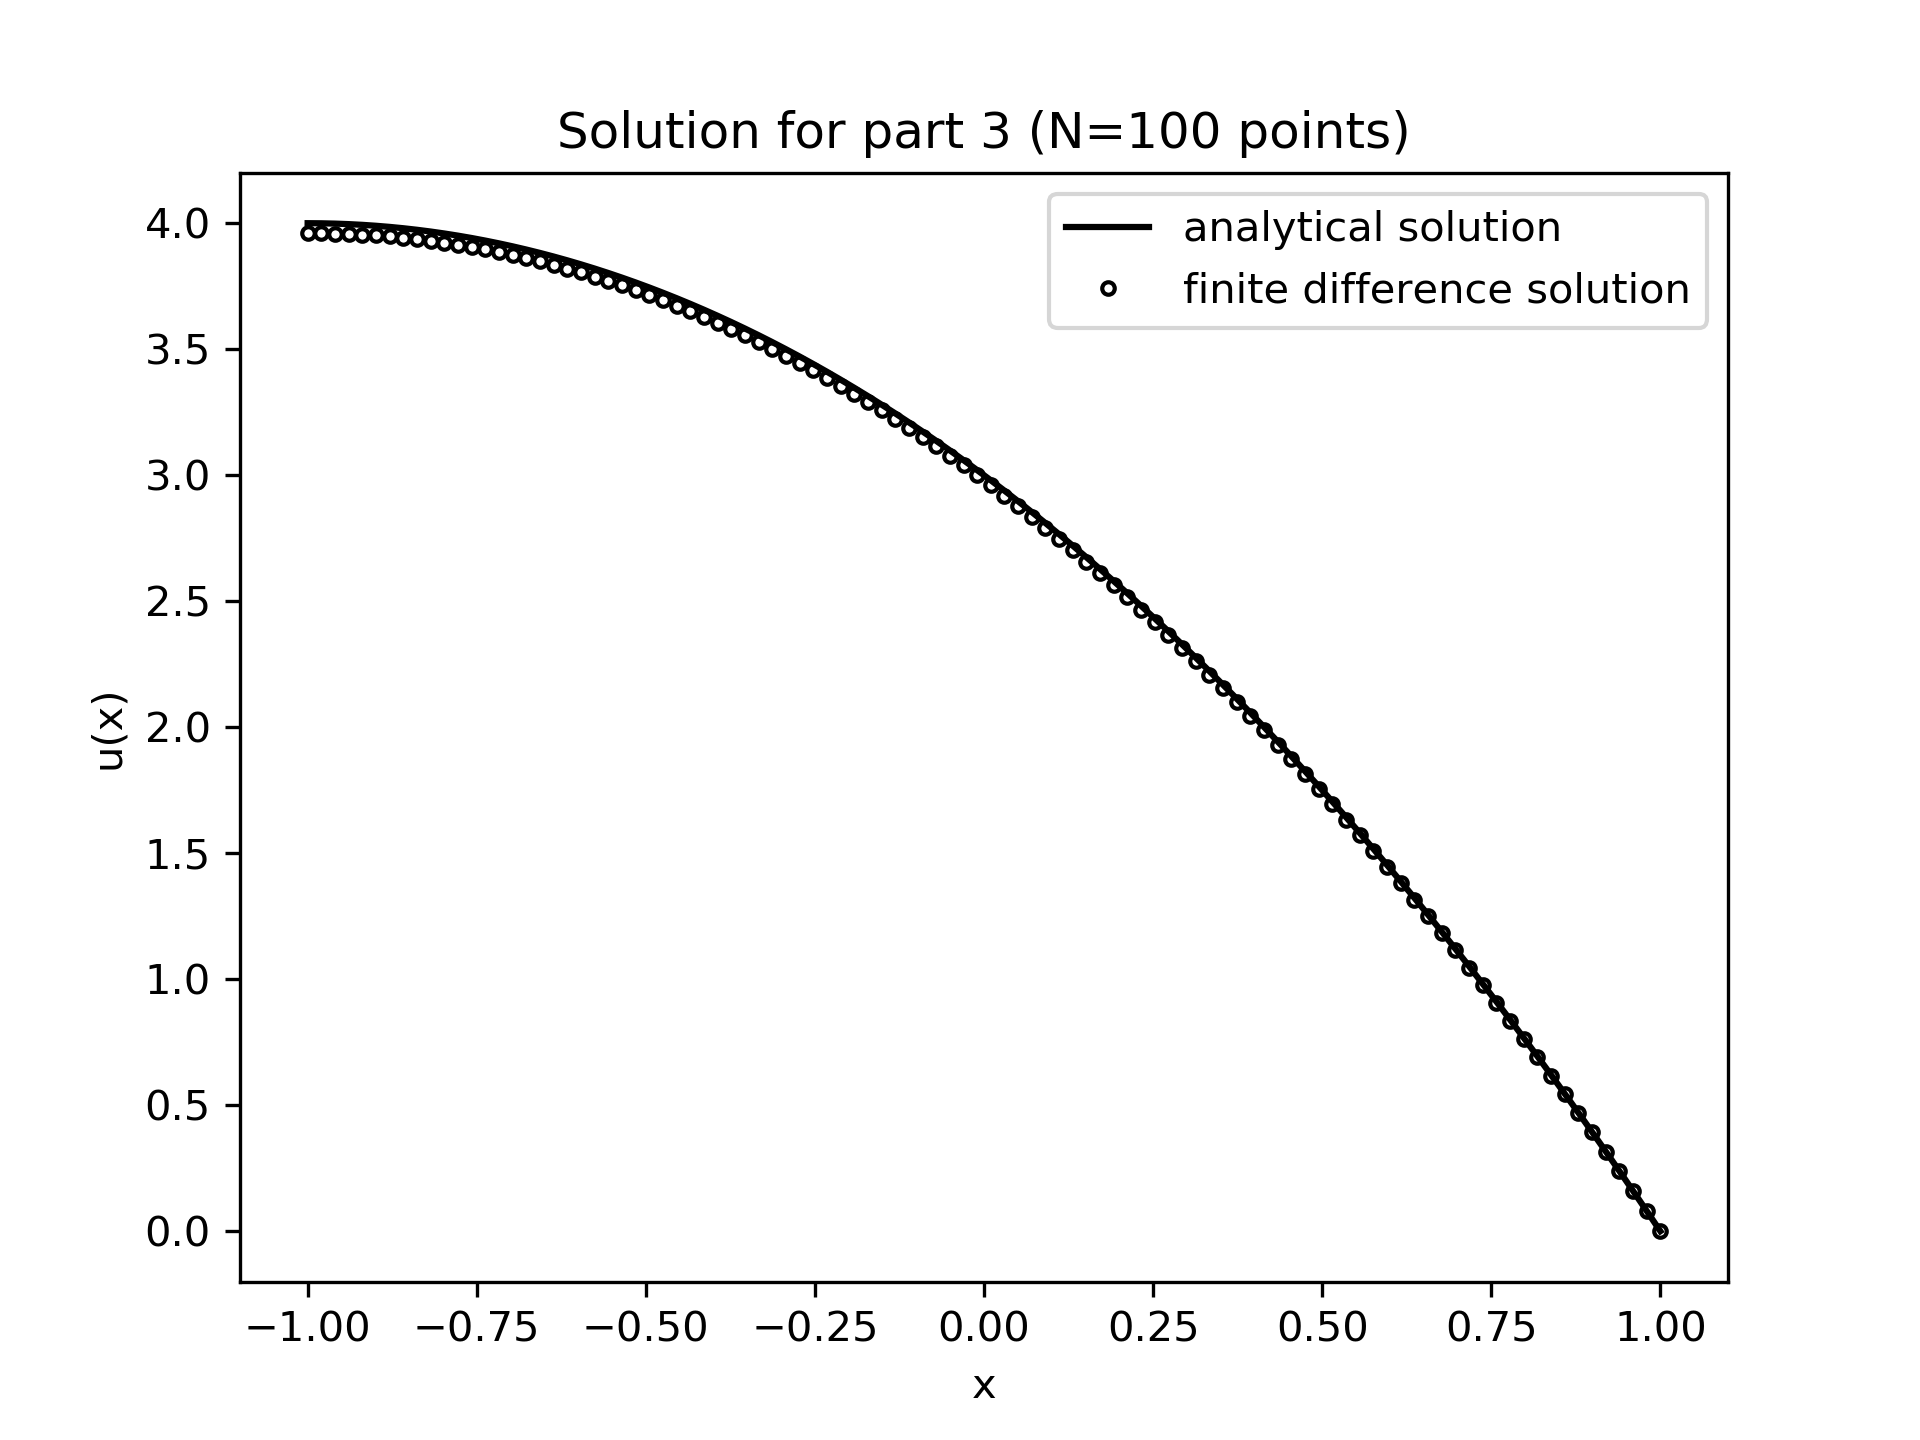
\includegraphics[scale=0.8]{part3.png}

\section{Bonus}
For the bonus section, we have the same setup as above except that the dirichlet boundary condition is $1$ instead of zero. Therefore, we would not strip off the last row and column as we did above but just use the equation $u_N = 0$ as the last row.

    \begin{bmatrix}
        -1 & 1 & 0 & \dots & 0 \\
        1 & -2 & 1 & \dots & 0 \\
        0 & 1 & -2 & 1 & \dots \\
        \vdots & \vdots & \vdots & \vdots & \ddots \\
        0 & 0 &\dots & 1 & -2 \\
        0 & 0 & \dots & 0 & 1 \\
    \end{bmatrix}
    \begin{bmatrix}
        u_0 \\
        u_1 \\
        \vdots \\
        u_{N-2} \\
        u_{N-1} \\
        u_N
    \end{bmatrix} 
    =
    \begin{bmatrix}
        0 \\
        -2 \\
        -2 \\
        -2 \\
        -2 \\
        1
    \end{bmatrix}

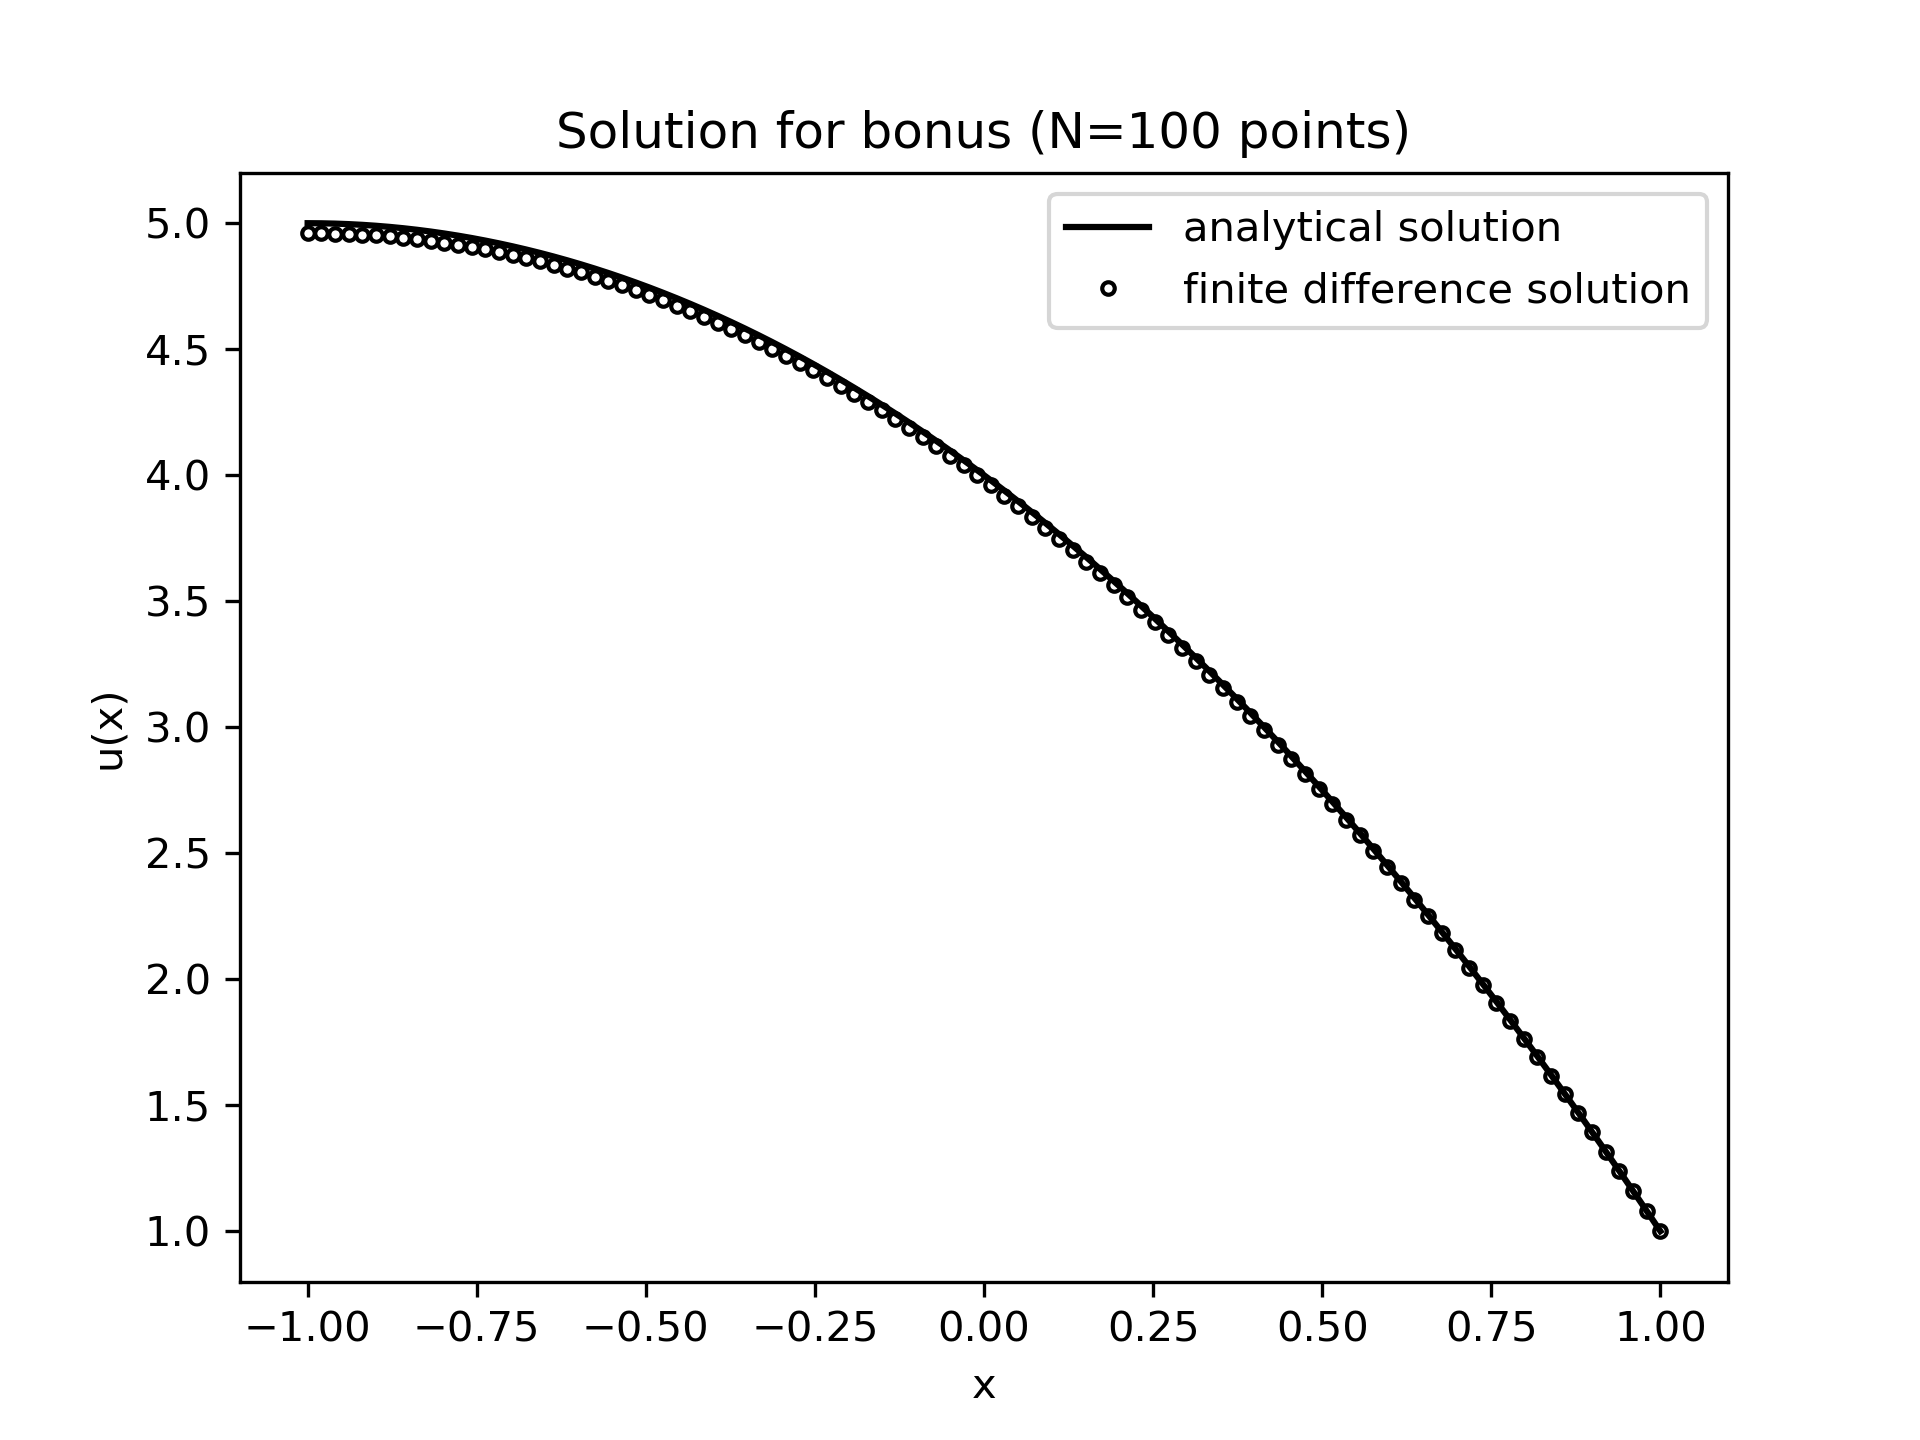
\includegraphics[scale=0.8]{bonus.png}

Since we are comparing our models to the analytical solution, we can be reasonably sure that our models are working correctly.

\end{document}
